\documentclass[tikz,border=0pt]{standalone}
\usepackage{mathptmx}
\usetikzlibrary{arrows.meta}
\definecolor{outline}{RGB}{0,99,163}
\definecolor{nodefill}{RGB}{237,247,255}
\newcommand{\figuretext}{\fontfamily{ptm}\fontsize{40bp}{46bp}\selectfont}
\begin{document}
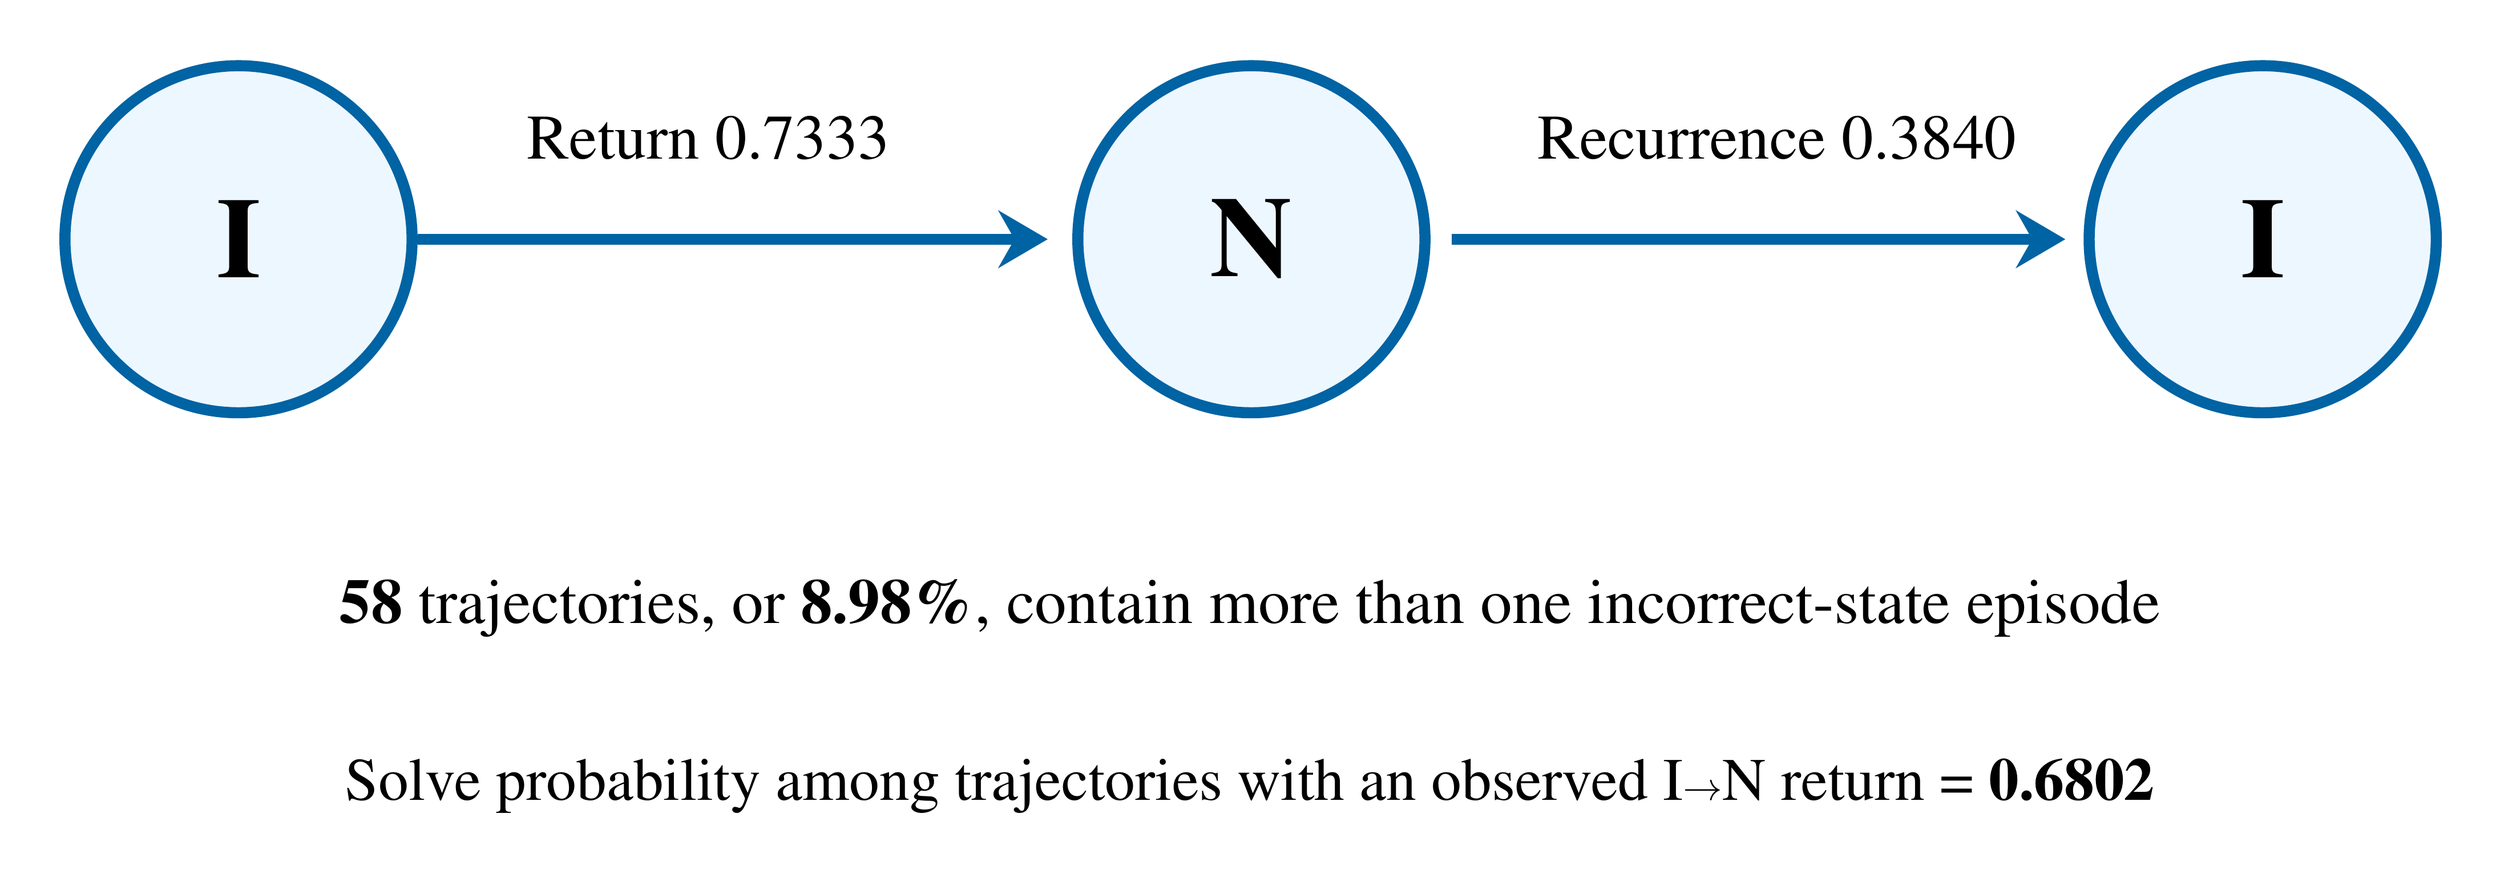
\begin{tikzpicture}[x=1bp,y=-1bp]
  \path[use as bounding box] (0,0) rectangle (1557,534);
  \fill[white] (0,0) rectangle (1557,534);
  % In the original layout, each node has an outer diameter of 226 bp.
  % This measurement includes the 7 bp outline and matches the original raster.
  \foreach \x/\label in {140.5/I,779.5/N,1417.5/I}{
    \draw[draw=outline,fill=nodefill,line width=7bp]
      (\x,141) circle[radius=109.5bp];
    \node[inner sep=0pt,font=\fontfamily{ptm}\fontsize{72bp}{78bp}\selectfont\bfseries]
      at (\x,141) {\label};
  }
  \draw[outline,line width=7bp,-{Stealth[length=31bp,width=36bp]}]
    (253.5,141) -- (651,141);
  \draw[outline,line width=7bp,-{Stealth[length=31bp,width=36bp]}]
    (906,141) -- (1293,141);
  \node[inner sep=0pt,font=\figuretext] at (437,77) {Return 0.7333};
  \node[inner sep=0pt,font=\figuretext] at (1111,77) {Recurrence 0.3840};
  \node[inner sep=0pt,font=\figuretext] at (778.5,374)
    {\textbf{58} trajectories, or \textbf{8.98\%}, contain more than one incorrect-state episode};
  \node[inner sep=0pt,font=\fontfamily{ptm}\fontsize{38bp}{44bp}\selectfont]
    at (778.5,486)
    {Solve probability among trajectories with an observed I$\rightarrow$N return = \textbf{0.6802}};
\end{tikzpicture}
\end{document}
